% This file was created with tikzplotlib v0.9.12.
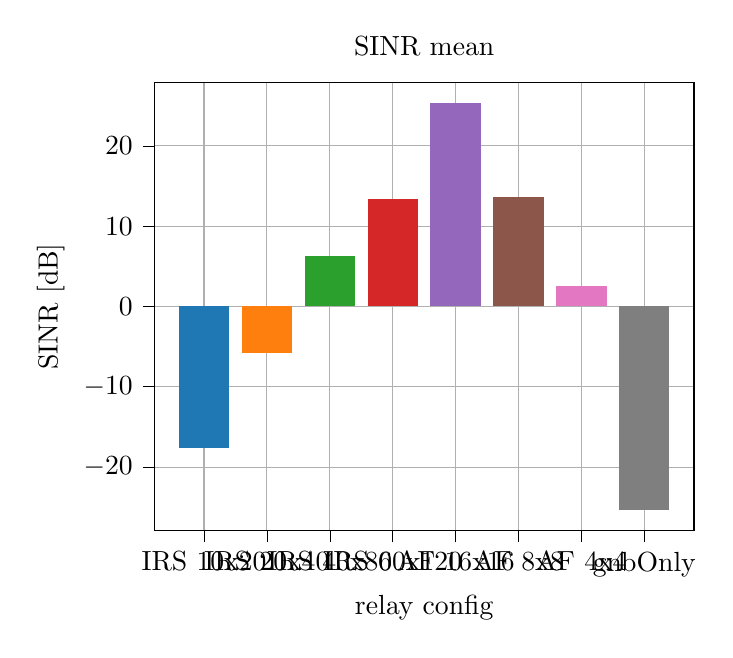
\begin{tikzpicture}

\definecolor{color0}{rgb}{0.12156862745098,0.466666666666667,0.705882352941177}
\definecolor{color1}{rgb}{1,0.498039215686275,0.0549019607843137}
\definecolor{color2}{rgb}{0.172549019607843,0.627450980392157,0.172549019607843}
\definecolor{color3}{rgb}{0.83921568627451,0.152941176470588,0.156862745098039}
\definecolor{color4}{rgb}{0.580392156862745,0.403921568627451,0.741176470588235}
\definecolor{color5}{rgb}{0.549019607843137,0.337254901960784,0.294117647058824}
\definecolor{color6}{rgb}{0.890196078431372,0.466666666666667,0.76078431372549}

\begin{axis}[
legend style={fill opacity=0.8, draw opacity=1, text opacity=1, draw=white!80!black},
tick align=outside,
tick pos=left,
title={SINR mean},
x grid style={white!69.0196078431373!black},
xlabel={relay config},
xmajorgrids,
xmin=-0.79, xmax=7.79,
xtick style={color=black},
xtick={0,1,2,3,4,5,6,7},
xticklabels={IRS 10x20,IRS 20x40,IRS 40x80,IRS 60x120,AF 16x16,AF 8x8,AF 4x4,gnbOnly},
y grid style={white!69.0196078431373!black},
ylabel={SINR [dB]},
ymajorgrids,
ymin=-27.8995208060441, ymax=27.9298981621926,
ytick style={color=black},
ytick={-30,-20,-10,0,10,20,30},
yticklabels={\ensuremath{-}30,\ensuremath{-}20,\ensuremath{-}10,0,10,20,30}
]
\draw[draw=none,fill=color0] (axis cs:-0.4,0) rectangle (axis cs:0.4,-17.5819049);
\draw[draw=none,fill=color1] (axis cs:0.6,0) rectangle (axis cs:1.4,-5.755327189);
\draw[draw=none,fill=color2] (axis cs:1.6,0) rectangle (axis cs:2.4,6.271295342);
\draw[draw=none,fill=color3] (axis cs:2.6,0) rectangle (axis cs:3.4,13.417793974);
\draw[draw=none,fill=color4] (axis cs:3.6,0) rectangle (axis cs:4.4,25.3921973);
\draw[draw=none,fill=color5] (axis cs:4.6,0) rectangle (axis cs:5.4,13.64638199);
\draw[draw=none,fill=color6] (axis cs:5.6,0) rectangle (axis cs:6.4,2.5703527);
\draw[draw=none,fill=white!49.8039215686275!black] (axis cs:6.6,0) rectangle (axis cs:7.4,-25.3618199438515);
\end{axis}

\end{tikzpicture}
